%++++++++++++++++++++++++++++++++++++++++
% Don't modify this section unless you know what you're doing!
\documentclass[letterpaper,11pt]{article}
\usepackage{tabularx} % extra features for tabular environment
\usepackage{float}
\usepackage{amsmath}  % improve math presentation
\usepackage{graphicx} % takes care of graphic including machinery
\usepackage[margin=1.3in,letterpaper]{geometry} % decreases margins
\usepackage{cite} % takes care of citations
\usepackage[final]{hyperref} % adds hyper links inside the generated pdf file
\usepackage{titlesec}
\usepackage{verbatim}
\usepackage{ragged2e}
\usepackage{amssymb}
\usepackage{tikz}
\usetikzlibrary{calc}
\tikzset{axis line style/.style={thin, gray, -stealth}}
\newcommand*{\TickSize}{2pt}
\setcounter{secnumdepth}{3}
\newtheorem{theorem}{Theorem}[section]
\newtheorem{property}{Property}[theorem]
\newtheorem{lemma}{Lemma}[theorem]

\makeatletter
\def\BState{\State\hskip-\ALG@thistlm}
\makeatother
\hypersetup{
	colorlinks=true,       % false: boxed links; true: colored links
	linkcolor=blue,        % color of internal links
	citecolor=blue,        % color of links to bibliography
	filecolor=magenta,     % color of file links
	urlcolor=blue
}
\newcommand\given[1][]{\:#1\vert\:}
\usepackage{listings}
\usepackage{array}
\usepackage{diagbox}
\usepackage{multicol}
\lstset{
  basicstyle=\ttfamily,
  mathescape
}
\usepackage{caption}
\usepackage{hyperref}

\usepackage{fvextra} % loads also fancyvrb
\usepackage{xpatch}

\DeclareMathVersion{ttmath}
\DeclareSymbolFont{latinletters}{OT1}{\ttdefault}{m}{n}
%\SetSymbolFont{latinletters}{ttmath}{OT1}{\ttdefault}{m}{n}
\SetSymbolFont{letters}{ttmath}{OML}{ccm}{m}{it}
\SetSymbolFont{symbols}{ttmath}{OMS}{ccsy}{m}{n}
\SetSymbolFont{largesymbols}{ttmath}{OMX}{ccex}{m}{n}

\newcommand{\changeletters}{%
  \count255=`A
  \advance\count255 -1
  \loop\ifnum\count255<`Z
    \advance\count255 1
    \mathcode\count255=\numexpr\number\symlatinletters*256+\count255\relax
  \repeat
  \count255=`a
  \advance\count255 -1
  \loop\ifnum\count255<`z
    \advance\count255 1
    \mathcode\count255=\numexpr\number\symlatinletters*256+\count255\relax
  \repeat
  \count255=`0
  \advance\count255 -1
  \loop\ifnum\count255<`9
    \advance\count255 1
    \mathcode\count255=\numexpr\number\symlatinletters*256+\count255\relax
  \repeat
}

\xapptocmd{\ttfamily}{\mathversion{ttmath}\changeletters}{}{}
%++++++++++++++++++++++++++++++++++++++++


\begin{document}

\title{\textbf{Practical Network Defense}\\ \bigskip \large First Assignment - University ``La Sapienza"}
\date{2020-13-04}
\author{\textbf{Group 27}: Nicola Bartoloni ******* - Valerio Trenta 1856471}
\maketitle

\section{Scope and Initial Considerations}
The scope of this assignment is to setup a \textbf{Virtual Private Network} through \textbf{OpenVPN} in \textbf{OPNSense} to allow three authenticated \textit{Road Warriors} to access the internal subnetworks of \textbf{ACME Co.}, and to grant the usage of a \textbf{proxy server} on machine located at \textbf{100.100.6.3} -  which corresponds to domain \textbf{proxy.acme.group27} to the very same authenticated internal clients of the network to reach the \textbf{WAN} outside the \textbf{Main Firewall}.\\
Since these tasks are going to allow connections from the outside - even if authenticated and thus probably secured - it is a good idea to make sure, as a first step, that every user on each of the internal machines is protected by a strong password, and we will probably also have to confirm that the SSH protocol on each machine behaves as we expect it to behave - some of the \textit{root} accounts are already disabled by SSH on some machines, but some are still accepting connections based on basic authentication.\\
The next paragraphs will only deal with the two services we want to setup in the target network - \textbf{VPN} and \textbf{proxy server}.

\newpage
\section{DHCP Setup}
How we performed the DHCP setup for the clients network.

\newpage
\section{Arpwatch tool configuration}
How we performed the configuration of the Arpwatch tool on the
Arpwatch machine.

\newpage
\section{Additional measures}
Configuring \textbf{Arpwatch} as described in the previous section is obviously not enough to guarantee a certain level of security in the target network, so we decided to take some extra measures that were not required by the assignment.\\
As a best practice, we chose to change the default passwords of every account in the machines of the network, and also the password for the admin account for the Internal Router has been changed. Strong, secure passwords on the \textbf{arpwatch machine} are a must-have in order for the monitoring system to actually be effective.\\
Apart from best practices, we needed to take into account possible threats such as \textbf{escalation of privilege} and \textbf{tampering} with the scripts' input in the \textbf{arpwatch machine}, so to make it difficult for an adversary to disrupt the monitoring system.

\subsection{Escalation of privilege on the Arpwatch machine}
This issue is pretty self-explanatory: in order for the script to be running, \textbf{root} has to be logged-in in the machine, meaning that an adversary could simply access it knowing its location (i.e., its IP address) and, being already logged-in as \textbf{root}, simply terminate the execution of the monitoring scripts, e.g. just by logging out of the account. Notice that this scenario could lead to even worse results for our system, such as the adversary being able to do basically everything he wants from the \textbf{arpwatch machine}. First measure we took was to actually launch the script at login such as, even when \textbf{root} or any other user logs out from bash, the monitoring script keeps running: this result was obtained through the \textbf{nohup} command being concatenated to the script when it is launched. This way, even if the user who executed the script logs out, it keeps running.\\
We do not need the \textbf{root} account to be logged in now to keep watching for possible spoofing attacks, but it is in general a best practice to execute scripts with the least possible privilege, so monitoring through \textbf{root} still seems a pretty bad idea. Indeed, if an adversary is granted access as \textbf{root}, he can still terminate the execution of the script, reboot or shut down the system. As a further security measure, a new account was created on the machine - \textbf{watchdog} - with no directory assigned and no privileges granted, so that it cannot create new files, edit old ones or execute files he does not own. This user basically doesn't own any file, but is given some specific permissions in order to perform the monitoring activity: first, he is able to \textit{only read} the arpwatch logs under \textit{/var/log/arpwatch.log}. Thanks to the \textbf{sudo} tool (by modifying \textit{visudo}), \textbf{watchdog} is able to launch from login the monitoring scripts - so that he can read and execute them, but not modify or delete them - and the \textbf{Python script} (so basically everything already existing under \textit{home} directory), which has been granted the privilege to actually create sockets and send packets through the \textbf{setcap} tool.\\
Also, the file \textbf{arp.dat} where the tool stores the arp entries is usually located at \textit{/var/lib/arpwatch}, but when run from \textbf{watchdog} arpwatch actually runs from directory \textbf{/}, so a new file \textbf{arp.dat} was created and owned by \textbf{root} in this directory. We tested and found out that \textbf{arpwatch}, when run by \textbf{watchdog}, uses this file and reads from it: this approach should be more secure since \textbf{watchdog} user cannot write to this second \textbf{arp.dat}, but \textbf{arpwatch} can still edit it while running without saving it, so it is able to store all the arp entries it needs there. When the script is eventually terminated by performing a rebot or a shut down from \textbf{root}, the file isn't saved, meaning the arp entries are lost and new stations will have to be re-discovered at new script startup, but this doesn't seem to affect badly the live detection, supposing a reboot of the machine will not occur frequently. Notice that every other action in the machine requires \textbf{watchdog} to input its own password, which was changed, and he cannot create new files without \textit{sudo} since he does not even own a directory - so, even if files executed in \textbf{Python} environment are actually able to send packets over the network, \textbf{watchdog} cannot create nor execute them: if he wants to, he needs to input its own password to be granted superuser privileges.\\
Furthermore, commands such as \textbf{reboot} and \textbf{shutdown} are disabled by default for \textbf{watchdog} without \textit{sudo} command, and even if the adversary logs out from this account, the monitoring script will keep running as previously mentioned.\\
Please notice also that \textit{sudo} is always requested to perform such actions - as, basically, every other action - since the \textit{sudoers} file was modified so that the default value for the \textit{timestamp$_$timeout} was set to \textbf{0}. At this point, the adversary cannot pose a threat to the machine that is worse than just killing the process related to the monitoring script, which at least can be prevented by logging in as \textbf{watchdog}, let the machine run the script and then log out - if passwords of the two accounts are not known to the adversary, the script's execution cannot be terminated.\\
Since the adversary is able to execute the monitoring scripts, he could provide \textbf{scapySendPacket.py} a bad input and exploit it to send packets over the network, which is an issue we deal with in the next subsection.\\

\subsection{Input validation in scapySendPacket.py}
The first, non-security related input validation phase requires the input to be at least two strings long. This is due to the fact that at least one string is required to match the target MAC address of the packet (the very first input string) and another one to be the payload, which we do not want to be empty. An error string will alert the user tampering with the input in this case, and the script will exit.\\
Another input validation mechanism was introduced in the Python script to actually prevent an adversary which gained access to a shell in the machine to abrirtarily send packets over the LAN exploiting this script itself.\\
Since we want \textit{scapySendPacket.py} to be triggered by new log lines in the arpwatch log file, before actually sending the requested payload to the specified MAC address, the script reads the log file and verifies that the payload itself is actually contained in this file.\\
This means that an adversary will not be able to send packets exploiting this script with an arbitrary payload, since the payload \textbf{must} be contained in the log file, else the script will terminate before sending the packet. Obviously, an adversary could still send its own packets by just setting as their input log lines that are already present in the log file, but at least it would be obvious to the sysadmin, and maybe also to the users receiving those packers, that such an attack is being performed: all the log lines - and thus, the payloads of the packet - contain \textit{date} and \textit{time}, so if they do not correspond to the date and time the packet was actually received, an user should still be able to tell that something's off.

\newpage
\section{Tests}
Tests that we run on both the two services aimed at verifying their correct behavior - i.e., that the two services were actually confgiured correctly so to be exploited as desired by non-malicious users - and that their setup does not hold a negative impact on the policy implemented in the previous assignment - i.e., the services can be only exploited by authenticated users under certain already mentioned conditions.

\subsection{Testing the VPN}
The \textbf{OpenVPN} service implemented on the \textbf{Main firewall} must be exploited only by an \textit{authenticated user} - that is, a user who owns \textit{three distinct credentials} in order to prove its identity and correctly gain access to the service. These three credentials are: the \textbf{.ovpn} file provided by the \textbf{OPNSense} portal correctly specifying the \textbf{valid cryptographic parameters} to authenticate the user on the \textbf{OpenVPN server}. This file holds the parameters that we previously showed, like port number, authentication type and the cryptographic functions to be arranged during the handshake between client and server, as pictured in \textbf{figure 7}.

\begin{figure}[!htb]
\centering
\begin{minipage}{.33\textwidth}
  \centering
  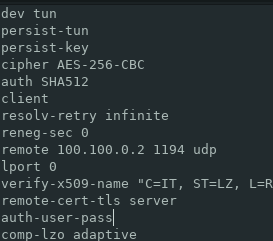
\includegraphics[width=1\textwidth]{ovpnParams.png}
  \caption[a]{Parameters in the .ovpn client file.}\label{fig:7}
\end{minipage}%
\end{figure}

Along with these parameters, the file also holds two different \textbf{keys}, one being the \textbf{certificate} for client to server authentication, the other being the \textbf{2048 bit OpenVPN static key} provided during the \textbf{TLS authentication}.\\
The other two credentials are the pair \textbf{(username, password)} specified under the settings of the \textbf{OPNSense} pannel - e.g., \textbf{Becca} as username and \textbf{password} as her password - and, furthermore, a \textbf{six characters token} provided by the \textbf{Google Authenticator}, which is a \textbf{One Time Password} different for each of the three users to be provided along the user's own static password during the basic authentication phase.\\
Once the \textbf{OpenVPN} terminates the intialization and the user authenticates successfully, he can exploit the new \textbf{tunnel} to gain access to the machines under the \textbf{Clients subnetwork} as requested by the assignment, through the \textbf{SSH} protocol on its own machine located in the \textbf{WAN} - once the \textbf{SSH} service has been enabled on the client's machines and routing has been appropriately configured on the local machine. This is the only operation that the \textbf{road warriors} are enabled to perform - they do not have access to the other subnetworks in the whole network, but we should stress the point that, once they gain access to one of the machines in the \textbf{Clients subnetwork}, they do have access to any other machine in the internal and DMZ subnet, which should actually be a desired feature.\\
\textbf{Figure 8} pictures the successful remote access of user \textbf{Becca} to the \textbf{kali machine} via the \textbf{OpenVPN service}. As far as we know, the only vulnerability that is introduced in the network with this service, is that now the \textbf{Main firewall} accepts connections on port \textbf{1194} on the \textbf{WAN} interface, and that the machines in the \textbf{Clients subnetwork} now accept connections with protocol \textbf{SSH} on \textbf{port 22} if and only if the request is coming from the \textbf{OpenVPN} tunnel - that is, only authenticated users should be actually able to login via \textbf{SSH} on those machines from the \textbf{WAN}.\\

\begin{figure}[!htb]
\centering
\begin{minipage}{.80\textwidth}
  \centering
  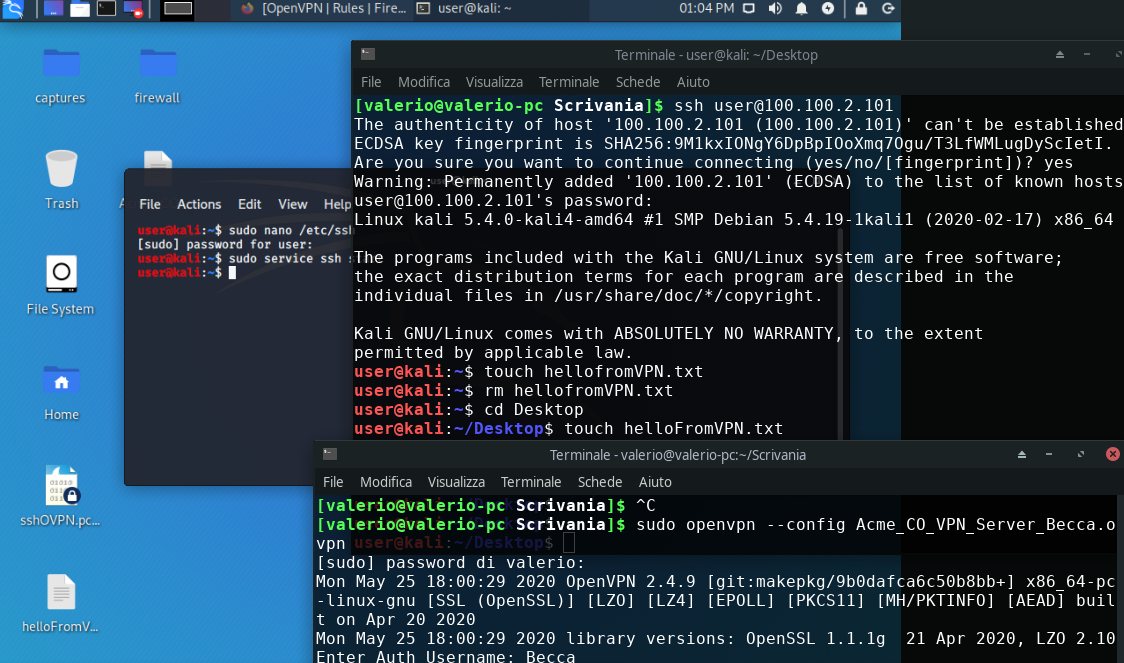
\includegraphics[width=1\textwidth]{OVPNaccessViaSSH.png}
  \caption[a]{User Becca accessing the Kali Machine via OpenVPN-SSH.}\label{fig:8}
\end{minipage}%
\end{figure}

\subsection{Testing the Proxy service}
We want the \textbf{squid proxy service} on the \textbf{proxy machine} to accept only users that have authenticated and are located in the \textbf{Clients subnetwork}, thus connections coming from a different subnetwork or the \textbf{WAN} are rejected a priori. In the \textbf{Kali machine}, we setup \textbf{Firefox browser} preferences so that it connects to the \textbf{proxy machine} requesting the \textbf{squid} service on port \textbf{3128} for every HTTP or HTTPS connection but those that have destination in the \textbf{Internal}, \textbf{External services} or \textbf{DMZ} subnetworks - \textit{manual configuration}. The figures below picture the desired behavior of both the services and the client's browser, which is now able to \textit{go out} in the \textbf{WAN} once the user is authenticated.\\

\begin{figure}[!htb]
\centering
\begin{minipage}{.5\textwidth}
  \centering
  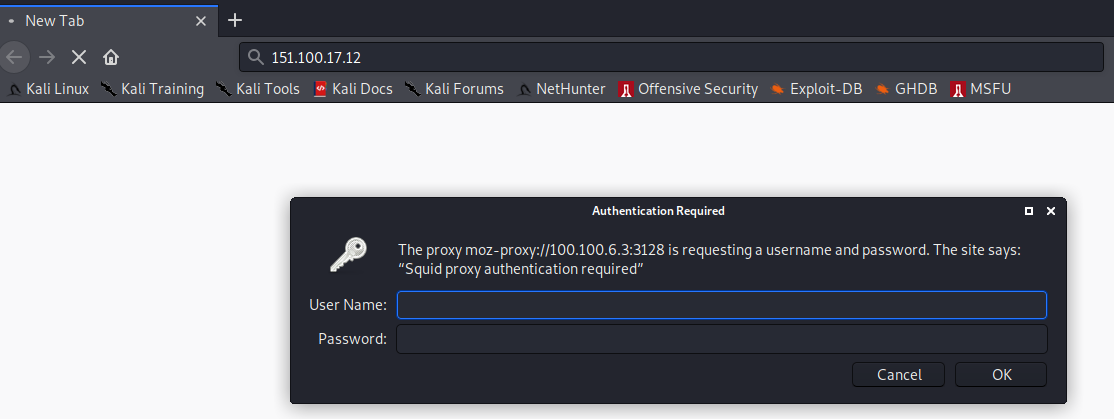
\includegraphics[width=1\textwidth]{proxyAuth.png}
  \caption[a]{Authentication procedure in the Kali machine's browser.}\label{fig:9}
\end{minipage}%
\begin{minipage}{.5\textwidth}
  \centering
  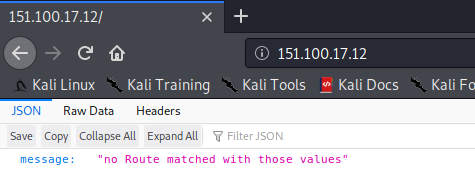
\includegraphics[width=1\textwidth]{proxyAuthed.png}
  \caption[a]{Successfully authenticated user can exploit proxy to display web pages outside of the network.}\label{fig:10}
\end{minipage}%
\end{figure}

\newpage
\section{Final remarks}
The testing phase showed us that the policy, if correctly interpreted, was implemented as specified by the assignment.\\
Some extra measures could have been taken, and they are very similar to the ones we have seen in the first assignment: we need to perform Linux hardening via sudo and hardening of the SSH protocol for all the machines in the DMZ and Internal Service subnetworks, and we need to change the default passwords for services such as \textbf{Zentyal} too and for users on the machines as well.\\
We should also stress the fact that, even if we found out that some of the machines had the SSH login via their \textit{root} account disabled by default, the scope of this assignment was to focus mainly on the \textbf{firewall rules} to be defined to achieve our goals and implement the given policy: this means that link$-$layer attacks were not taken into consideration, and this may be a critical vulnerability in our network. indeed, notice that every machine can be accessed through SSH or other protocols by any other machine on its same subnetwork - i.e., \textit{dc} can access \textit{logserver} through any protocol. This is because the rules we defined to implement our policy are placed on the two firewall$-$routers, which obviously do not handle packets exchanged between hosts in the same subnetwork: to overcome this issue, probably some extra rules should also be defined locally on each machine via \textit{iptables} - but this was out of our scope for this assignment.\\
We should also mention the fact that the \textbf{UDP} protocol was chosen to implement the \textbf{rsyslog} service, which could be also implemented through \textbf{TCP} protocol - commonly considered more secure - and maybe forced to exploit secure channels. Again, our goal here was to enable the service and enforce the policy via firewall rules, but we should stress the fact that just by exploiting TCP, this service may be hardened.\\
Also, as a last step, when the whole configuration going on in these assignments is over, we should at least enable only one machine in the \textbf{Clients} subnetwork - the \textbf{Kali} machine, probably - to connect via HTTP service to the two routers, for administration and practical reasons, so as we mentioned in the previous paragraphs, the rule enabling these connections should be actually disabled as a last step.

\newpage

\begin{thebibliography}{9}
\bibitem{Aggarwal}\href{https://web.cs.hacettepe.edu.tr/~aykut/classes/spring2013/bil682/supplemental/outlierbook.pdf}{\em Just a placeholder.}
\end{thebibliography}
\end{document}
